\documentclass[17pt]{extbook} % 14, 17, 20
\usepackage{cmap} % Для кодировки PDF
\usepackage[utf8]{inputenc} % Кодировка входа
\usepackage[encoding,filenameencoding=utf8]{grffile} %Нормально читаем кодировку файловой системы
\usepackage[T2A]{fontenc} % Кодировка выхода
\usepackage[russian]{babel} % Локаль
\usepackage{pscyr} % Крутые русские шрифты (http://scon155.phys.msu.su/~swan/cyrtug2000.pdf)
\usepackage[babel=true]{microtype} % Точный подгон текста
\usepackage[paperwidth=210mm, paperheight=210mm,includefoot]{geometry} % Геометрия
\geometry{margin=2cm}

\makeatletter  % Костыль для кириллицы в input
    \let\old@input\input
    \renewcommand\input[1]{%
        \expandafter\old@input{"\detokenize{#1}"}%
    }
\makeatother

\makeatletter
\def\input@path{{texts/}}
\makeatother

\newcommand{\inputText}{\input {texts/}}

\usepackage{graphicx} % Картинки
\graphicspath{{pictures/}}
\DeclareGraphicsExtensions{.pdf,.png,.jpg}

\frenchspacing % Одинарный пробел в конце предложений
\renewcommand{\familydefault}{far} % Шрифт (tex\latex\pscyr\pscyr.sty)


\usepackage{fancyhdr} % Колонтитулы
\pagestyle{fancy}
\fancyhf{} 			% Очистить
\cfoot{\thepage}	% Добавить номер
\renewcommand{\headrulewidth}{0pt} % Без линии
\fancypagestyle{plain}{ % Для страниц с заголовками раздела chapter
	\fancyhf{}
	\cfoot{\thepage}	% Добавить номер
}



\usepackage[explicit]{titlesec}  % Заголовки
\titleformat{\chapter}[drop]{}{}{0pt}{}
\titlespacing*{\chapter}{0pt}{-20pt}{0pt}

\titleformat{\part}{}{}{0pt}{}
\titlespacing*{\part}{0pt}{0pt}{0pt}



\setlength\parindent{0pt}
\newcommand\X{\par\noindent---~}

\usepackage{epigraph}


\begin{document} %-----------------------------------------------------

\chapter{002. Викинги}

\begin{figure}[p!]
\center{\includegraphics[scale=0.5]{Викинги.png}}
\center{Борода лучше её отсутствия}
\label{fig:image}
\end{figure}

\epigraph{Робот, которому грустно, и Викинги}

\X Привет, робот.
\X Привет, Викинги.
\X Как настроение?
\X Мне грустно.
\X Не отчаивайся. Хочешь пограбить и поубивать вместе?
\X Давай.
\par
Некоторое время робот грабил караваны, убивал женщин и насиловал мужчин. Викинги одобрительно поддерживал его деятельность. После кровавого веселья и хмельного пира робот и Викинги снова встретились.
\par
\X Привет, робот.
\X Привет, Викинги.
\X Ну что, робот, ты вдоволь награбил и наубивал?
\X Думаю, да.
\X Как ощущения?
\X Мне грустно.


\chapter{004. Создатель}

\begin{figure}[p!]
\center{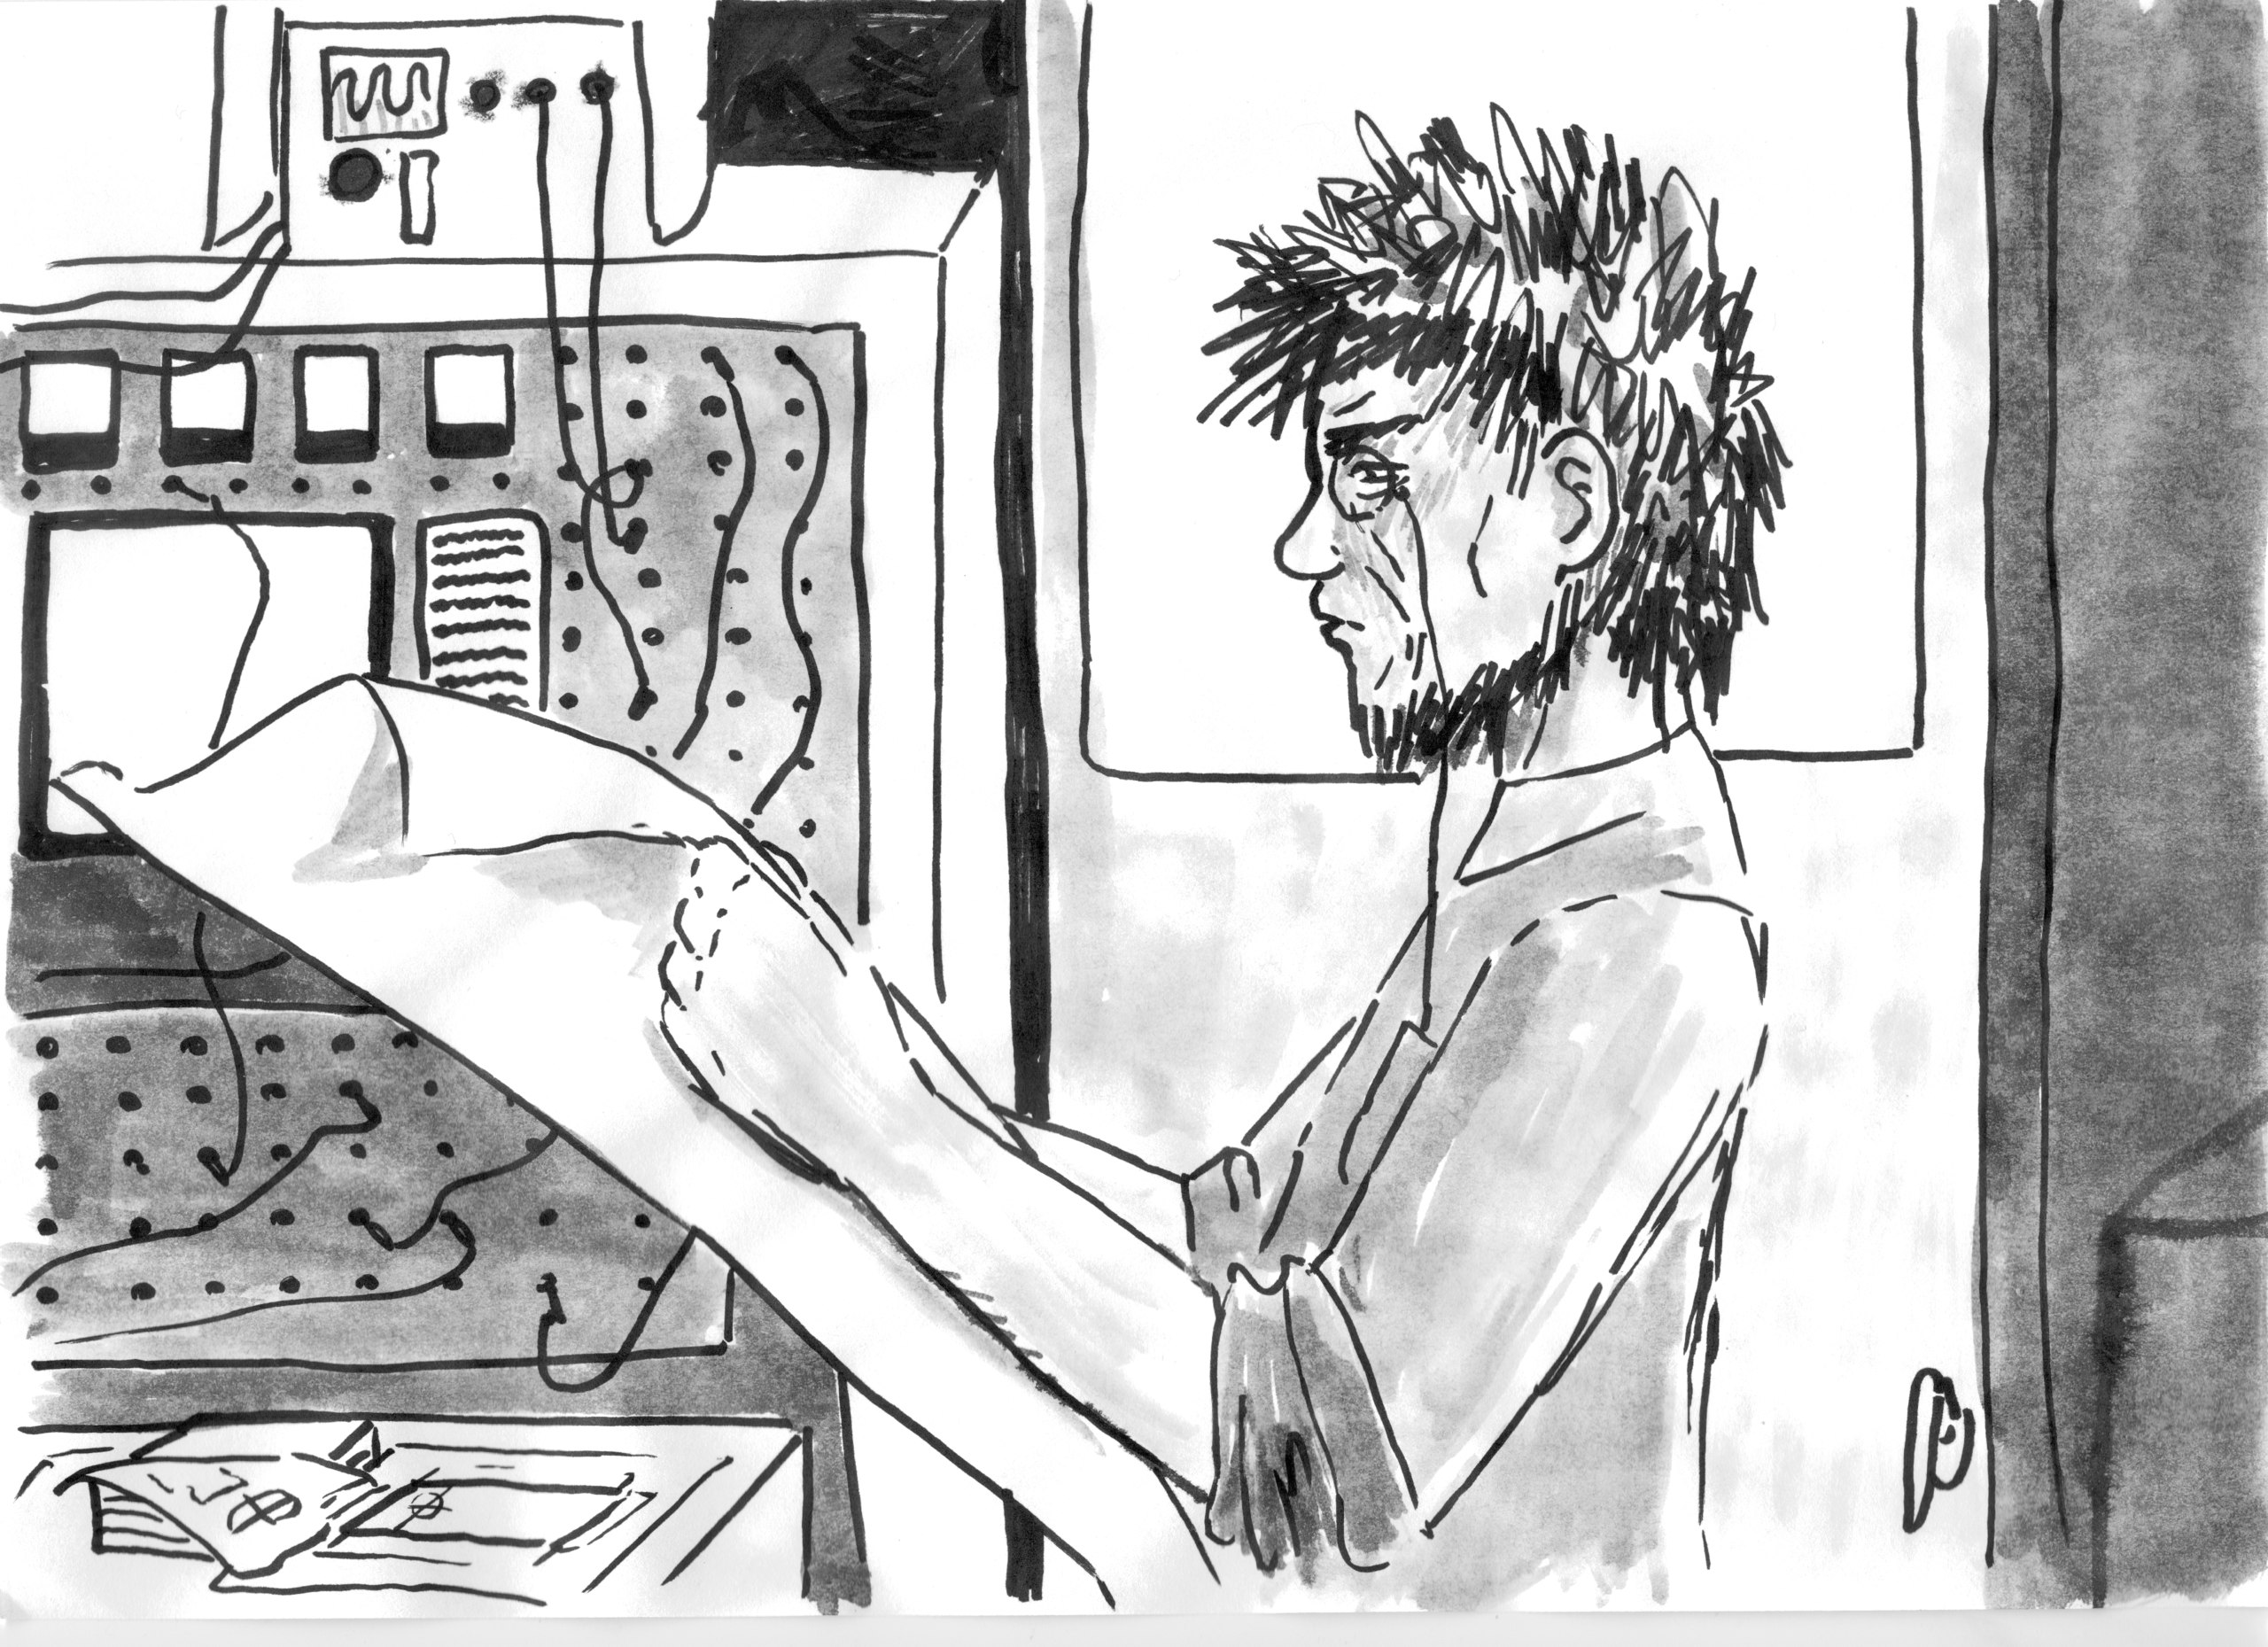
\includegraphics[scale=1.5]{Создатель.jpg}}
\center{Все мы порой что-то создаём}
\label{fig:image}
\end{figure}

\epigraph{Робот, которому грустно, и Создатель}

\begin{dialog}
\X Привет, робот.
\R Привет, Создатель.
\X Как ты себя ощущаешь?
\R Мне грустно.
\X Так и должно быть.
\end{dialog}

\begin{monolog}
Робот ушёл. Долгое время скитался по миру. Не найдя ответа, он решил вернуться к Создателю.
\end{monolog}
	
\begin{dialog}
\X Привет, робот.
\R Привет, Создатель.
\X Тебе всё ещё грустно?
\R Да, мне всё ещё грустно.
\X Так будет всегда.
\R Но зачем?
\X Потому что ты Робот, которому грустно. Помни об этом.
\end{dialog}

\end{document}